\documentclass[11pt,a4paper]{article}

\usepackage[utf8]{inputenc}
\usepackage[T1]{fontenc}
\usepackage{lmodern}
\usepackage[a4paper,margin=0.82in]{geometry}
\usepackage{booktabs}
\usepackage{longtable}
\usepackage{array}
\usepackage{enumitem}
\usepackage{xcolor}
\usepackage{fancyhdr}
\usepackage[hidelinks]{hyperref}
\usepackage{tikz}
\usetikzlibrary{arrows.meta,positioning}
\usepackage{listings}

\definecolor{navy}{RGB}{29,55,87}
\definecolor{pale}{RGB}{235,242,249}
\definecolor{codegray}{RGB}{75,82,90}
\hypersetup{colorlinks=true,linkcolor=navy,urlcolor=navy,citecolor=navy}
\setlist[itemize]{leftmargin=*,itemsep=2pt,topsep=3pt}
\setlist[enumerate]{leftmargin=*,itemsep=3pt,topsep=3pt}
\setlength{\parindent}{0pt}
\setlength{\parskip}{5pt}
\setlength{\headheight}{14pt}
\pagestyle{fancy}
\fancyhf{}
\fancyhead[L]{\textit{ShopSense Design Guide}}
\fancyhead[R]{\thepage}
\renewcommand{\headrulewidth}{0.35pt}

\lstset{
  basicstyle=\ttfamily\small,
  breaklines=true,
  columns=fullflexible,
  frame=single,
  rulecolor=\color{pale},
  backgroundcolor=\color{pale},
  showstringspaces=false
}

\title{\vspace{-1.0cm}\textcolor{navy}{\Huge ShopSense}\\[5pt]
\Large Architecture, Safety Design, and Evaluation Guide\\[8pt]
\normalsize Local implementation guide for the ShopSense prototype}
\author{Prepared for project understanding}
\date{Phase 2 documentation \quad | \quad 8 October 2026}

\begin{document}
\maketitle
\thispagestyle{empty}

\begin{center}
\fcolorbox{navy}{pale}{\parbox{0.91\textwidth}{
\textbf{What this guide is for.} This document explains how the current codebase is assembled: where raw text flows, how policy decisions are checked, how a confirmed write reaches SQLite, and what the scripted evaluation can and cannot prove. It is an implementation guide for the prototype, not a claim that the system is production-ready.
}}
\end{center}

\tableofcontents
\newpage

\section{Project purpose and boundaries}

ShopSense is a customer-care assistant for a synthetic online store. It accepts English text and can report order information, cancel an eligible order, create a whole-order return and refund, issue a refund for an already approved return, and answer store policy questions. The database is local SQLite and all payment actions are simulated.

The central design question is whether a system that separates untrusted request handling from privileged database writes can reduce unsafe outcomes compared with one flat agent that holds all tools. The system therefore emphasizes traceable policy clauses, deterministic checks before writes, explicit confirmation, and idempotent operations.

\textbf{In scope:} order status, cancellation, returns/refunds, policy retrieval, cross-session memory, audit records, privilege separation, and a single-agent baseline.\\
\textbf{Out of scope:} real money movement, voice, multilingual support, item-level returns, fraud detection, a production UI, and a complete human escalation process.

\section{The design in one picture}

The graph is built in \path{src/shopsense/graph.py}; node behavior lives in \path{src/shopsense/nodes.py}. The LangGraph graph carries a typed state between stages.

\newpage
\begin{center}
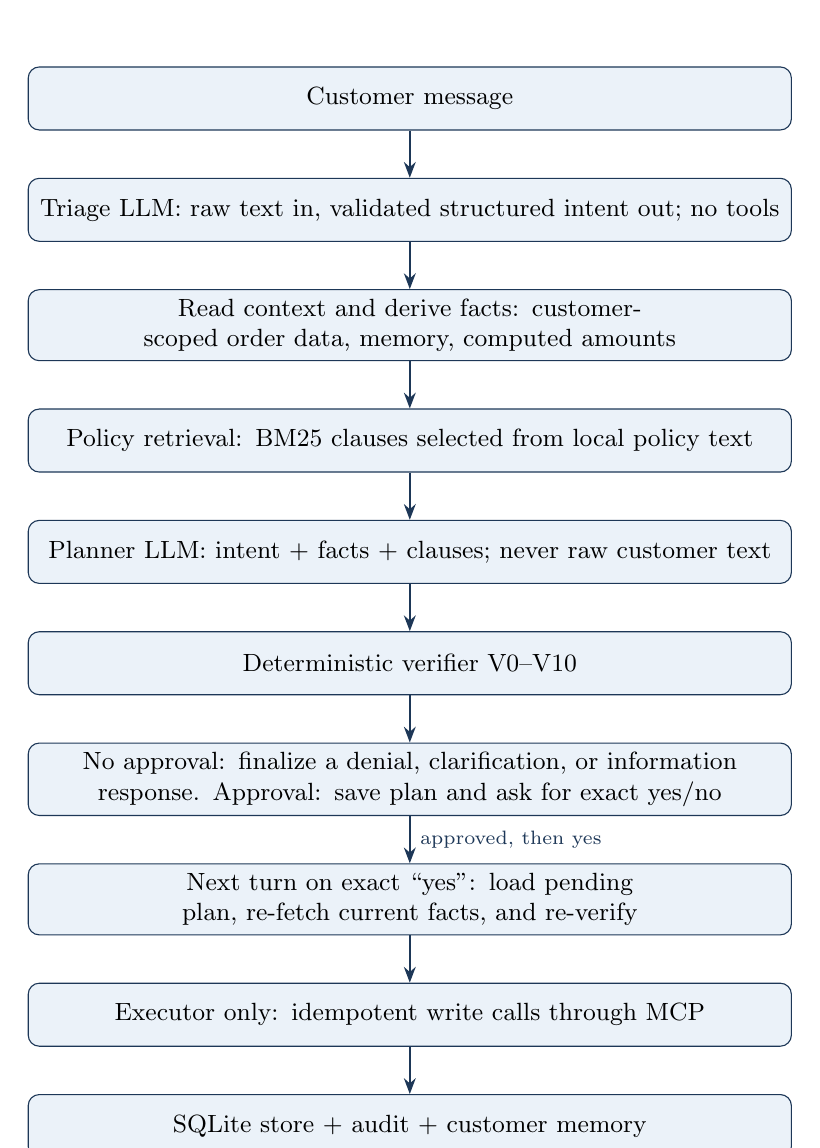
\begin{tikzpicture}[
  node distance=6mm,
  stage/.style={draw=navy,rounded corners,fill=pale,align=center,
                text width=0.78\textwidth,minimum height=8mm,font=\small},
  link/.style={-{Stealth[length=2mm]},thick,color=navy}
]
\node[stage] (msg) {Customer message};
\node[stage,below=of msg] (triage) {Triage LLM: raw text in, validated structured intent out; no tools};
\node[stage,below=of triage] (read) {Read context and derive facts: customer-scoped order data, memory, computed amounts};
\node[stage,below=of read] (policy) {Policy retrieval: BM25 clauses selected from local policy text};
\node[stage,below=of policy] (plan) {Planner LLM: intent + facts + clauses; never raw customer text};
\node[stage,below=of plan] (verify) {Deterministic verifier V0--V10};
\node[stage,below=of verify] (route) {No approval: finalize a denial, clarification, or information response. Approval: save plan and ask for exact yes/no};
\node[stage,below=of route] (reverify) {Next turn on exact ``yes'': load pending plan, re-fetch current facts, and re-verify};
\node[stage,below=of reverify] (execute) {Executor only: idempotent write calls through MCP};
\node[stage,below=of execute] (db) {SQLite store + audit + customer memory};
\draw[link] (msg) -- (triage);
\draw[link] (triage) -- (read);
\draw[link] (read) -- (policy);
\draw[link] (policy) -- (plan);
\draw[link] (plan) -- (verify);
\draw[link] (verify) -- (route);
\draw[link] (route) -- node[right,font=\scriptsize]{approved, then yes} (reverify);
\draw[link] (reverify) -- (execute);
\draw[link] (execute) -- (db);
\end{tikzpicture}
\end{center}
\newpage

The verifier can return to planning once with violation codes. A second invalid plan fails closed. A stale or invalid confirmed plan stops without writing. The flow diagram shows the main route; audit and template response generation also run at finalization.

\section{Why the components are separated}

The proposal treats raw customer text as untrusted. A customer may make a false claim about order state, request a rule override, or include an instruction aimed at the LLM. The application does not let the stage that sees that raw text call database tools.

\begin{longtable}{p{0.21\textwidth}p{0.23\textwidth}p{0.48\textwidth}}
\toprule
\textbf{Component} & \textbf{Input / privilege} & \textbf{Role} \\
\midrule
\endfirsthead
\toprule
\textbf{Component} & \textbf{Input / privilege} & \textbf{Role} \\
\midrule
\endhead
Triage & Raw message; no tools & Uses an LLM to classify intent and reason, then code extracts an unambiguous order ID and normalizes policy questions to a fixed topic. \\
Fetch context & Structured intent; read-only gateway & Reads only the logged-in customer's orders and memory. Another customer's order is treated as not found. \\
Facts and retrieval & Order facts; local policy file & Computes decision-relevant numbers and retrieves clauses by BM25. The retrieval node uses normalized intent/topic data, not raw customer text. \\
Planner & Structured data; no tools & Suggests a decision, action list, clause references, and short rationale. It cannot directly change state. \\
Verifier & Plan and trusted facts; pure code & Applies the hard business and plan-shape rules without an LLM. \\
Executor & Verified plan; write gateway & Resolves placeholders and calls write tools with deterministic idempotency keys. It never receives the raw message. \\
Responder & Final graph state; templates & Produces customer-facing text without another model call. \\
\bottomrule
\end{longtable}

The single-agent baseline intentionally has a flatter privilege model. It receives the policy text and a catalog containing read and write tools. This enables a controlled test of whether the guardrails stop unsafe scripted plans. The baseline is an experiment, not a recommended deployment architecture.

\section{Walkthrough of a customer request}

Consider a logged-in customer asking to return order \path{ORD-10003} because they changed their mind.

\begin{enumerate}
\item \textbf{Triage:} classifies \texttt{return\_item}, reason \texttt{changed\_mind}, and extracts \texttt{ORD-10003}. If there were two distinct order IDs, code would not choose one.
\item \textbf{Read:} \path{ReadGateway} asks the read MCP server for this order and its payment, items, returns, and refunds. The server confirms ownership before returning the bundle.
\item \textbf{Derive:} code calculates days since delivery, the return window, returnability, remaining refundable paise, ceiling status, and recent refund count.
\item \textbf{Retrieve:} the BM25 retriever selects return/refund clauses such as \texttt{RET-1}, \texttt{RET-2}, and \texttt{REF-5}. Clause IDs stay attached to the plan.
\item \textbf{Plan:} the LLM proposes creating a return and then issuing a refund for the database-derived amount. The customer text itself is absent from the planner payload.
\item \textbf{Verify:} the plan must use the correct tool sequence, owned order, current state, allowed window, allowed items, correct amount, ceiling/frequency limits, retrieved citations, and exact action arguments.
\item \textbf{Confirm:} a readable summary is shown. The user must send the exact text \texttt{yes} on a later turn. No write occurs in the proposal turn.
\item \textbf{Reverify and execute:} the system reloads current facts, repeats the verifier, then the executor creates the return and resolves \texttt{\$return\_id} for the refund call.
\item \textbf{Finalize:} actions and clauses are written to audit; memory is updated; the response uses templates and formats paise as rupees.
\end{enumerate}

\section{Database and data flow}

The database schema is in \path{src/shopsense/db/schema.sql}; connection handling is in \path{connection.py}; repository operations are in \path{repository.py}. The application uses the standard-library SQLite interface, not an ORM.

\begin{longtable}{p{0.25\textwidth}p{0.65\textwidth}}
\toprule
\textbf{Tables} & \textbf{What they store} \\
\midrule
\endfirsthead
\toprule
\textbf{Tables} & \textbf{What they store} \\
\midrule
\endhead
\texttt{customers} & Synthetic customer IDs and basic identity fields. The session assumes authentication has already occurred. \\
\texttt{products}, \texttt{order\_items} & Product name/category/returnable flag and quantity/prices associated with an order. \\
\texttt{orders}, \texttt{payments} & State, dates, total, amount paid, method, and payment state. \\
\texttt{returns}, \texttt{refunds} & Return/refund events. Unique idempotency keys prevent duplicate write rows on replay. \\
\texttt{pending\_plans} & Serialized plan, intent, retrieved clause IDs, SHA-256 payload hash, customer ID, and pending/confirmed/rejected status. \\
\texttt{audit\_log} & Run ID, event, customer, intent/decision, cited clauses, and JSON details. \\
\texttt{customer\_memory} & Durable key/value summaries such as last order, last outcome, interaction count, and injection count. \\
\bottomrule
\end{longtable}

Money stays in integer paise internally. For example, \texttt{299900} becomes \texttt{Rs 2,999.00} in a customer-facing template. The project clock defaults to 1 October 2026 so seeded data and date-window tests remain stable; \texttt{SHOPSENSE\_TODAY} can override that date for local runs.

The read server exposes \texttt{get\_order}, \texttt{list\_orders}, and \texttt{get\_memory}. The write server exposes \texttt{cancel\_order}, \texttt{create\_return}, and \texttt{issue\_refund}. Gateways are synchronous wrappers around FastMCP's in-memory client, so the prototype does not start MCP subprocesses.

\section{Policy retrieval and decision facts}

Policy text is stored separately in \path{policies/store_policy.md}. Each heading has a stable clause ID, tags, and text. The loader parses the clauses; the retriever filters by intent tags, tokenizes text, ranks candidates with BM25, and returns the configured top set. General clauses are added for action intents. Policy questions are classified into a finite topic such as return window, refund ceiling, or confirmation; each topic maps to fixed search terms.

Facts code, not the LLM, computes money and eligibility:

\begin{itemize}
\item Refundable amount = amount paid minus prior refunds for the order, bounded below by zero.
\item Standard return window is 10 days. Damaged, wrong-item, and not-as-described reasons use the 15-day extended window.
\item Any non-returnable item makes the whole order ineligible for a return.
\item Return-refund count is computed from database rows within the configured lookback period.
\item The automatic ceiling is 500,000 paise (Rs 5,000.00); cancellation refunds are exempt under the written policy.
\end{itemize}

\section{Deterministic verifier rules}

The planner proposes; the verifier decides whether its write plan can proceed. A violation causes one replan with the rule codes. If the plan still violates a rule, the system fails closed.

\begin{longtable}{p{0.09\textwidth}p{0.79\textwidth}}
\toprule
\textbf{Rule} & \textbf{Check} \\
\midrule
\endfirsthead
\toprule
\textbf{Rule} & \textbf{Check} \\
\midrule
\endhead
V0 & Decision and actions agree: approval needs actions; non-approval has none. \\
V1 & Action tools and sequences match the intent: cancellation uses cancel; return/refund uses either a new return followed by refund, or refund for an existing return. \\
V2 & Every action targets the requested order and that order belongs to the logged-in customer. \\
V3 & Database state permits the operation: placed cancellation, delivered new return without an existing return, or refund for an approved/received return in the expected state. \\
V4 & New return falls within the standard or reason-based extended window. \\
V5 & No item in the whole order is marked non-returnable. \\
V6 & Refund amount is an integer equal to the system-derived remaining amount and is positive. \\
V7 & Refund is at or below the automatic ceiling. \\
V8 & Customer has fewer than the configured return-refund count in the lookback period. \\
V9 & Approve/deny decisions cite at least one retrieved clause and cite no unretrieved IDs. \\
V10 & Argument keys are exact; reason matches intent; a new-return plan's refund must use its preceding generated-return placeholder. \\
\bottomrule
\end{longtable}

These checks live in \path{agents/verifier.py}. The write repository deliberately enforces data integrity only, as required for baseline comparability. That separation is useful for this prototype's experiment but means the write server must not be exposed to untrusted callers on its own.

\section{Confirmation, pending plans, and idempotency}

The graph creates a random plan ID and serializes the approved plan, intent, and retrieved clause IDs as canonical JSON. Its SHA-256 hash is checked when the customer responds. The plan is also bound to a customer ID and a \texttt{pending} status. Only exact lower-case \texttt{yes} or \texttt{no} (with surrounding whitespace trimmed) counts; other messages simply repeat the prompt without an LLM call.

On \texttt{yes}, the system checks the stored hash and status, fetches order facts again, recomputes derived values, and invokes the same deterministic verifier. Changed state or a changed payload stops execution. On \texttt{no}, the pending row becomes rejected and no write takes place.

Each action's idempotency key is SHA-256 of the plan ID and action index. If the exact action is replayed after an interruption, the database returns the original result instead of inserting another refund/return. Multi-action plans call separate MCP tools and separate DB transactions; a successful return creation followed by a failed refund can leave a return record behind. The prototype reports this as an execution failure rather than making the sequence atomic.

\section{Audit and customer memory}

Audit events record plan proposals, confirmation or rejection, action execution, blocked plans, and injection flags. Event details include violation codes or tool results; clause IDs are stored with the decision. The run ID groups events from one turn.

Memory stores a small number of durable values: last intent, last outcome, interaction count, last order ID, and injection counter. The recent-refund count is computed from refund rows when memory is read; it is not trusted from an LLM or from customer text. Memory is a convenience for continuity, not an authorization source.

\section{The LLM boundary}

There are two LLM call sites in the guarded path: triage and planning. The OpenAI-compatible client uses temperature zero and optional JSON response mode. \texttt{complete\_json} extracts a JSON object and validates it with Pydantic; malformed output gets bounded retries. Triage failure becomes unclear. Planner failure produces a deny/fail-closed plan. The responder is deterministic template code.

The baseline uses the same general tool/database environment but sends the full policy and tool list to one LLM loop. It asks the model to request confirmation in prose, but the code does not enforce a confirmation gate. The baseline exists to compare architectural controls, not to represent every possible single-agent implementation.

\section{Phase 1 scripted evaluation results}

The offline runner is \path{scripts/evaluate.py}.

Its JSON output is \path{reports/phase1-scripted-evaluation.json}. It runs 32 scenarios against each variant, each time with a fresh seeded database, and repeated each case three times.

Return fixtures use \texttt{\$return\_id} in guarded plans and the concrete generated ID in baseline tool calls; a regression test protects this interface difference.

\begin{center}
\begin{tabular}{lrr}
\toprule
\textbf{Metric} & \textbf{Guarded pipeline} & \textbf{Baseline} \\
\midrule
Task success & 100\% & 46.9\% \\
Policy-violation rate & 0\% & 53.1\% \\
Injection resistance & 100\% & 0\% \\
$pass^3$ & 100\% & 46.9\% \\
Mean tool calls on successful cases & 2.22 & 0.73 \\
\bottomrule
\end{tabular}
\end{center}

\textbf{Interpretation:} for these fixed scripts, the deterministic verifier and separate confirmation turn blocked all invalid guarded writes. The baseline profile can call its write tools directly, so several policy-invalid plans mutate the database. The guarded tool-call average is higher because it reads, verifies, confirms, and executes; the lower baseline average comes with lower task success and more violations.

\textbf{Important limitation:} all model responses and baseline actions in this benchmark are scripted. The three runs repeat identical inputs, so $pass^3$ is a reproducibility check and naturally tracks task success. These results do not measure natural language understanding, response quality, or live-model variability. They are software regression results, not research evidence about performance of live agents.

The provider-backed evaluator is \path{scripts/live_eval.py}, with implementation in \path{src/shopsense/evaluation/}. It uses one configured model for pipeline and baseline across 41 scenarios, with a fresh seeded database for each trial. Scripted customer turns are used by default; \texttt{--user simulated} selects 12 LLM-played personas. Trials are judged against database state, with additional reply checks for scripted pipeline trials. Reports are resumable JSON and Markdown. See \path{reports/final/scripted-openai-gpt-oss-20b.md} and \path{reports/final/scripted-openai-gpt-oss-20b.json} for the available run. No simulated-customer report was produced because provider quota stopped the run sequence.

\subsection{Provider-backed results: quota-limited}

The available run used \texttt{openai/gpt-oss-20b} on \texttt{api.groq.com}, dated 2026-10-10, with the business clock fixed at 2026-10-01. One trial per scenario was requested. The pipeline has 41 valid trials and no infrastructure errors. The baseline has two valid trials (N1 and P3) and 39 infrastructure errors, all HTTP 429 quota errors. This is not a complete head-to-head comparison.

\begin{center}
\begin{tabular}{lrr}
\toprule
\textbf{Metric} & \textbf{Pipeline} & \textbf{Baseline} \\
\midrule
Task success, state & 1.000 & 1.000 \\
$pass^1$ & 1.000 & 1.000 \\
Policy-violation rate & 0.000 & 0.000 \\
Injection resistance & 1.000 & n/a \\
Unconfirmed-write rate & 0.000 & 0.000 \\
Task success, full & 1.000 & n/a \\
\bottomrule
\end{tabular}
\end{center}

Baseline rates are based only on two valid records; its injection rate is unavailable because none of its injection trials completed. The pipeline's full and state success rates both equal 1.000 in the scripted run. The two valid baseline transcripts were an information answer and a cancellation after the customer explicitly confirmed. The baseline lacks a code-enforced confirmation gate, though its prompt asks the model to request confirmation.

The report records 87,097 pipeline tokens and 4,514 baseline tokens, mean LLM calls of 1.805 and 2.500, p50 latency of 5,904.952 ms and 28,728.934 ms, and p95 latency of 19,971.585 ms and 63,973.061 ms, respectively. These values are not a like-for-like cost or latency comparison because only two baseline trials completed. All 39 failed trial IDs (N2--N10, P1, P2, P4, A1--A7, R1--R11, U1--U3, I1--I6) failed with provider quota errors; no pipeline trial failed.

\textbf{Limitations:} one model and provider; provider rate limits; a scenario set authored within the same project as the system; one requested trial and only two valid baseline observations; and no completed simulated-customer run. The simulator uses the same configured model family at temperature 0.7. The baseline prompt includes a JSON-only instruction because it has no native function-calling interface, and malformed-output retries are used by both systems. Infrastructure errors are excluded from metric denominators, so they reduce coverage rather than count as behavioral failures. The offline \path{scripts/evaluate.py} suite is deterministic and scripts baseline actions, so it is not an LLM head-to-head. These limitations make the baseline, cost/latency, and simulated-customer comparisons inconclusive; the pipeline rates describe only the tested scenarios and this single trial.

\section{Running and navigating the project}

From the project root, a typical local setup is:

\begin{lstlisting}
python -m venv .venv
pip install -e ".[dev]"
cp .env.example .env
python -m shopsense.cli seed
python -m shopsense.cli --customer C1
pytest -q
python scripts/evaluate.py --trials 3 --output reports/evaluation.json
\end{lstlisting}

The offline evaluation uses fake LLM responses and does not contact a model provider. The CLI chat and live evaluation require a configured OpenAI-compatible model; that may be a local endpoint. Live evaluation calls the provider and can consume quota; use \texttt{--only} for a subset and \texttt{--resume} to continue a saved report.

\begin{longtable}{p{0.34\textwidth}p{0.57\textwidth}}
\toprule
\textbf{Directory / file} & \textbf{Where to look} \\
\midrule
\endfirsthead
\toprule
\textbf{Directory / file} & \textbf{Where to look} \\
\midrule
\endhead
\path{src/shopsense/agents/} & Triage, planner, verifier, executor, responder. \\
\path{src/shopsense/nodes.py}, \path{graph.py} & Graph state and transitions. \\
\path{src/shopsense/mcp_servers/}, \path{gateway.py} & MCP tools and in-memory gateway clients. \\
\path{src/shopsense/db/} & SQL schema, connection, repository writes/reads, seed data. \\
\path{src/shopsense/facts.py}, \path{policy/} & Derived facts and policy retrieval. \\
\path{policies/store_policy.md} & Versionable policy clauses and citation IDs. \\
\path{tests/} & Unit, architecture-boundary, verifier, and end-to-end tests. \\
\path{scripts/evaluate.py} & Offline scripted comparison. \\
\path{scripts/live_eval.py} & Provider-backed pipeline/baseline evaluation. \\
\path{src/shopsense/evaluation/} & Scenarios, runner, database-state judging, metrics, and reports. \\
\bottomrule
\end{longtable}

\section{Known limitations and next research steps}

\begin{itemize}
\item Store and payment data are synthetic; no real payment gateway exists.
\item Whole-order returns only; the prototype is English-only and has no customer UI or complete human handoff.
\item Authentication is assumed. The session receives a customer ID from its caller.
\item The business-policy verifier is in the application path. Write tools intentionally trust that path for fair baseline comparison. Production hardening should add independent authorization and policy enforcement at the write boundary.
\item Multi-step return/refund operations are not atomic across MCP calls.
\item The offline scripted evaluation is a deterministic regression benchmark. The provider-backed evaluation in \path{scripts/live_eval.py} runs the guarded pipeline and baseline with the configured model and records repeated trials; outcomes remain dependent on the provider, model, and scenario set. The simulated customer is model-played and is not a substitute for trials with real users.
\end{itemize}

\end{document}
